\documentclass[10pt, a4paper]{exam}
\usepackage{graphicx}
\usepackage[a4paper, total={7in, 9.5in}]{geometry}
\usepackage[normalem]{ulem}
\usepackage{amsmath}
\renewcommand\ULthickness{1.0pt}   
\setlength\ULdepth{1.3ex}

\begin{document}


	\noindent
	\begin{minipage}[l]{0.1\textwidth}
		\noindent
		
\includegraphics[width=2.8\textwidth]{ESCUDO.png}
	\end{minipage}
\hfill
\begin{minipage}[c]{0.8\textwidth}
	\begin{center}
		{\large  Departamento de Ingeniería civil y Agrícola\par
		\large	Facultad de Ingeniería	\par
	% \large \textbf{Taller propiedades de los fluidos}	\par
    \large \textbf{Laboratorio No. 2 \\ Conservaci\'on de la cantidad de movimiento: Resalto hidr\'aulico}	\par
} %%%%% NOMBRE DEL PROFESOR 
	\end{center}
\end{minipage}
\par
\vspace{0.2in}
\noindent
    \uline{Mecánica de fluidos [2015966]	\hfill 2022-II	}
\par 
\vspace{0.15in}
\noindent

%%%%%%%%%%%%%%%%%%%%%%%%%%%%%
\section{Normas del Laboratorio}
\begin{itemize}
    \item \textbf{Grupos}: Los grupos seran de 5 o 6 estudiantes m\'aximo. Los estudiantes son libres de organizar los grupos.
    \item \textbf{Duraci\'on}: Cada grupo tendr\'a una hora aproxim\'adamente  para realizar el laboratorio.
    \item \textbf{Material}: Es necesario vestir bata o overol para la realizaci\'on del laboratorio. Este atuendo puede ser de cualquier color o fabricante. Traer calculadora, l\'apiz y papel.
\end{itemize}


\section{Objetivo}
Este laboratorio tiene como fin estudiar la conservaci\'on de la cantidad de movimiento en un resaldo hidr\'aulico. Algunos objetivos espec\'ificos propuestos son:
\begin{itemize}
\item Determinar la fuerza ejercida por el flujo sobre la compuerta aguas arriba del resalto.
\item Determinar la fuerza y la energ\'ia espec\'ifica antes y despu\'es del resalto hidr\'aulico. Calcular las perdidas de energ\'ia ($\Delta E$).
\item Graficar las curvas de fuerza espec\'ifica ($F_e$) y energ\'ia espec\'ifica ($E_e$) para el resalto.
\item Determinar la posici\'on de la profundidad cr\'itica $y_c$ en el resalto.
\end{itemize}

\section{Metodolog\'ia}
Este laboratorio se har\'a en un canal de flujo a superficie libre de pendiente horizontal y secci\'on rectangular constante. Dicho canal est\'a provisto de una compuerta rectangular localizada a la entrada del canal y unas rejillas al final del canal que se usar\'an para generar un resalto hidr\'aulico est\'able para un caudal $Q$ (ver figura~\ref{can}). La metodolog\'ia para la toma de datos es la siguiente:
\begin{figure}[h]
    \centering
    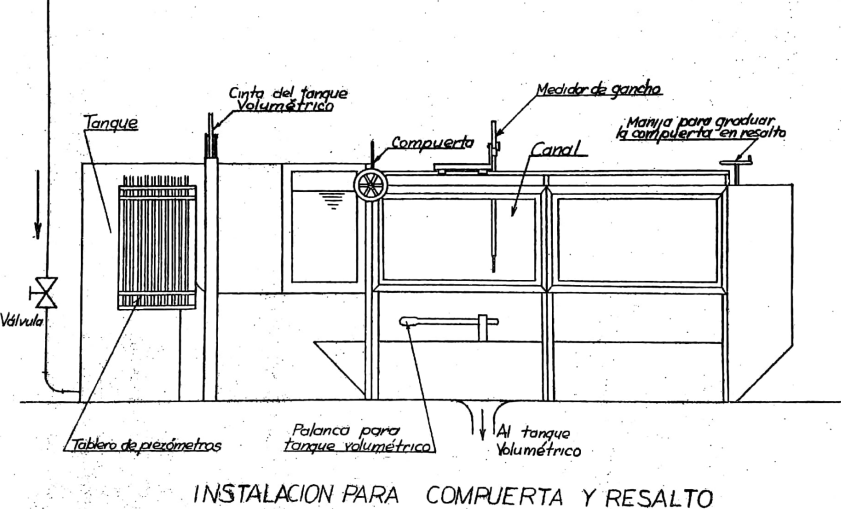
\includegraphics[width=\textwidth]{canalRH.png}
    \caption{Esquema del canal del laboratorio para (sacado de Guias del Laboratorio de Hidr\'aulica, UNAL, 1994)}
    \label{can}
\end{figure}

\begin{enumerate}
\item Para un caudal determinado, estabilizar el resaldo hidr\'aulico utilizando la compuerta y las rejillas al final del canal.
\item Una vez estabilizado el resalto, tomar las presiones usuando los piezometros:
\begin{enumerate}
\item A lo largo del fondo del canal
\item Sobre la compuerta
\end{enumerate}
\item Como medida alternativa a las presiones de los piezometros en el fondo del canal, medir las profundidades de la lamina de agua antes, despues y en el resalto utilizando la aguja vertical. Tomar 10 profundidades en total.  
\item Usando el tanque volum\'etrico y cron\'ometro, determinar el caudal que pasa por el canal. 
\end{enumerate}

\section{Resultados esperados}
Usando los datos tomados de acuerdo con la metodolog\'ia, realizar los siguientes c\'alculos.
\begin{enumerate}
\item Calcular el caudal $Q$ que fluye en el canal utilizando:
$$
Q = V/\Delta t
$$
donde $V$ es el volumen acumulado en el tanque volum\'etrico durante un $\Delta t$.

\item Graficar las l\'inea de energ\'ia (LE) y la l\'inea de gradiente hidr\'aulico (LGH).

\item Para el volumen de control comprendido entre una secc\'on 1 aguas arriba de la compuerta y una seccion 2 aguas abajo de la compuerta en donde no hay p\'erdidas de energ\'ia, estimar el caudal $\hat{Q}$, utilizando la ecuaci\'on de Bernoulli:
$$
\frac{P_1}{\gamma} + z_1 + \frac{V_1^2}{2g} = \frac{P_2}{\gamma} + z_2 + \frac{V_2^2}{2g}
$$
Si el nivel de referencia es el fondo del canal, $z_1 = z_2 =0$  y si de acuerdo con la ecuaci\'on de continuidad $\hat{Q}=Q_1 = Q_2 $, la ecuaci\'on anterior se transforma en:
$$
\frac{P_1}{\gamma} - \frac{P_2}{\gamma}  = + \frac{\hat{Q}^2}{2g} \left(\frac{1}{A_2} - \frac{1}{A_1}\right)
$$
despejando $\hat{Q}$,
$$
\hat{Q} = \sqrt{\frac{2g\left(\frac{P_1}{\gamma} - \frac{P_2}{\gamma}\right)}{\left(\frac{1}{A_2} - \frac{1}{A_1}\right)}}
$$
donde $\frac{P_1}{\gamma} =y_1$ y $\frac{P_2}{\gamma} =y_2$ son las profundidades de agua en la secci\'on 1 y 2 respectivamente. Si $A_1 = y_1 b$ y $A_2 = y_2 b$, donde $b$ es el ancho del canal, la ecuaci\'on anterior es:
$$
\hat{Q} = \sqrt{\frac{2g\left(y_1 - y_2\right)}{\left(\frac{1}{y_2 b} - \frac{1}{y_1 b}\right)}}
$$
$y_1$ y $y_2$ las profundidades pueden ser determinadas usando los piez\'ometros de agua. Una v\'ez calculado $\hat{Q}$ comparar con el $Q$ medido (real).

\item Determinar la fuerza de reacci\'on $R_x$ de la compuerda a la fuerza din\'amica del flujo utilizando la ecuaci\'on de conservaci\'on de la cantidad de movimiento para el canal rectangular en el volumen de control de la compuerta:
$$
\sum F_x = \rho Q \left( Vx_2 -  Vx_1 \right)
$$
en donde $Vx_2$ es la velocidad aguas abajo de la compuerta (a la salida del volumen de control) y $Vx_1$ es la velocidad aguas arriba de la compuerta (a la entrada del volumen de control) en $x$, y $\sum F_x$ es la sumatoria de las fuerzas externas actuantes sobre el volumen de control:
$$
\sum F_x = R_x + F_1 - F_2 = \rho Q \left( Vx_2 -  Vx_1 \right)
$$
donde $F_1 = \gamma \frac{y_1^2 b}{2}$ y $F_2 = \gamma \frac{y_2^2 b}{2}$ son las fuerzas hidroest\'aticas en la secci\'on 1 y 2, respectivamente. Reemplazando en la ecuaci\'on tenemos que:
$$
R_x = \rho Q \left( Vx_2 -  Vx_1 \right) - \gamma \frac{y_1^2 b}{2} + \gamma \frac{y_2^2 b}{2}
$$

\item En el volumen de control comprendido entre una secci\'on antes 1 y  despues 2 del resalto, determinar la fuerza espec\'ifica 
$$
F_e = \frac{\gamma b y^2}{2} + \frac{\gamma Q V}{g}
$$
en 1 y en 2. Partiendo de la igualdad:
$$
\frac{\gamma b y_1^2}{2} + \frac{\gamma Q V_1}{g} = \frac{\gamma b y_2^2}{2} + \frac{\gamma Q V_2}{g}
$$
se puede llegar a: 
$$
\frac{y_2}{y_1} = \frac{1}{2}\left[ \sqrt{1+8F_{R_1}^2} -1 \right]
$$
donde:
$$
F_R = \frac{V}{\sqrt{gh}}
$$
pruebe la valid\'ez de la relaci\'on $\frac{y_2}{y_1}$.

\item Determinar las p\'erdidas de energ\'ia en el resalto $\Delta E = E_{e_1} - E_{e_2}$, donde la energ\'ia espec\'ifica $E_e$ es:
$$
E_e  = y + \frac{v^2}{2g}
$$
Pruebe la valid\'ez de la expresi\'on te\'orica:
$$
\Delta E = \frac{(\hat{y}_2 - y_1)^3}{4y_1 y_2}
$$
donde $\hat{y}_2$ es la profundidad en 2 estimada usando la relaci\'on $\frac{y_2}{y_1}$ data anteriormente.
\item Si la longitud del resalto $L_R$ es te\'oricamente igual a:
$$
L_R = 5(y_2 - y_1)
$$
pruebe la valid\'ez de esta expresi\'on.

\item Usando las profundidades tomadas antes, a lo largo y despu\'es del resalto, pintar en una misma gr\'afica las curvas de $E_e$ vs $y$ y $F_e$ vs $y$, donde $y$ son las abcisas. Se\~nale la p\'erdida de energ\'ia $\Delta E$ en la gr\'afica.

\item Calcular la profundidad cr\'itica $y_c$ usando:
$$
y_c = \sqrt[3]{\frac{q^2}{g}}
$$
donde $q$ es caudal por unidad de ancho y ubicarla en la gr\'afica anterior de $F_e$ vs $y$. Determinar aproxim\'adamente a que distancia de la secci\'on 1 (entrada al resalto) se encuentra la $y_c$.

\end{enumerate}

\section{Informe}
El informe de laboratorio debe contener las siguientes secciones: 
\begin{enumerate}
    \item Introducci\'on: Breve texto para poner en contexto el laboratorio.
    \item Metodolog\'ia: Describe el procedimiento de toma de datos y el seguido para obtener los resultados.
    \item Resultados: Presenta los resultados del labotorio. Dado el caso, se deben incluir gr\'aficas y tablas que resuman los resultados.
    \item Conclusiones: Se discuten all\'i las conclusiones obtenidas a partir de los resultados. Se hacen las comparaciones del caso.
    \item Referencias: Incluir las referencias consultadas.
\end{enumerate}
El informe no debe contener como ma\'aximo 4 hojas escritas en ambas caras en espacio sencillo, tama\~no de fuente 11 y a doble columna. 

\end{document}



